\section{Requisiti soddisfatti}
\subsection{Tabella del soddisfacimento dei requisiti}
\begin{table}[hp]
\centering
\begin{tabular}{|c|c|c|}
\hline
ID requisito & Soddisfacimento nell'architettura & Soddisfacimento nel codice \\ \hline
R0F1         & SODDISFATTO                       & SODDISFATTO                \\ \hline
R0F2         & SODDISFATTO                       & SODDISFATTO                \\ \hline
R0F3         & SODDISFATTO                       & SODDISFATTO                \\ \hline
R0F4        & SODDISFATTO                       & SODDISFATTO                \\ \hline
R0F5        & SODDISFATTO                       & SODDISFATTO                \\ \hline
R0F6        & SODDISFATTO                       & SODDISFATTO                \\ \hline
R2F7        & SODDISFATTO                       & NON SODDISFATTO                \\ \hline
R2F8        & SODDISFATTO                       & NON SODDISFATTO                \\ \hline
R2F9        & SODDISFATTO                       & NON SODDISFATTO                \\ \hline
R2F10        & SODDISFATTO                       & NON SODDISFATTO                \\ \hline
R2F11        & SODDISFATTO                       & NON SODDISFATTO                \\ \hline
R2F13        & SODDISFATTO                       & NON SODDISFATTO                \\ \hline
R2F14        & SODDISFATTO                       & NON SODDISFATTO                \\ \hline
R0F15        & SODDISFATTO                       & SODDISFATTO                \\ \hline
R0F16        & SODDISFATTO                       & SODDISFATTO                \\ \hline
R0F17        & SODDISFATTO                       & SODDISFATTO                \\ \hline
R0F18        & SODDISFATTO                       & SODDISFATTO                \\ \hline
R0F19        & SODDISFATTO                       & NON SODDISFATTO                \\ \hline
R2F20        & SODDISFATTO                       & NON SODDISFATTO                \\ \hline
R2F21        & SODDISFATTO                       & NON SODDISFATTO                \\ \hline
R2F22        & SODDISFATTO                       & NON SODDISFATTO                \\ \hline
R0F23        & SODDISFATTO                       & SODDISFATTO                \\ \hline
R0F24        & SODDISFATTO                       & SODDISFATTO                \\ \hline
R2F25        & SODDISFATTO                       & NON SODDISFATTO                \\ \hline
R0F26        & SODDISFATTO                       & SODDISFATTO                \\ 
\hline
\end{tabular}
\caption{Requisiti soddisfatti}
\end{table}
\clearpage

\subsection{Grafici sui requisiti soddisfatti}
\begin{figure}[hp]
\centering
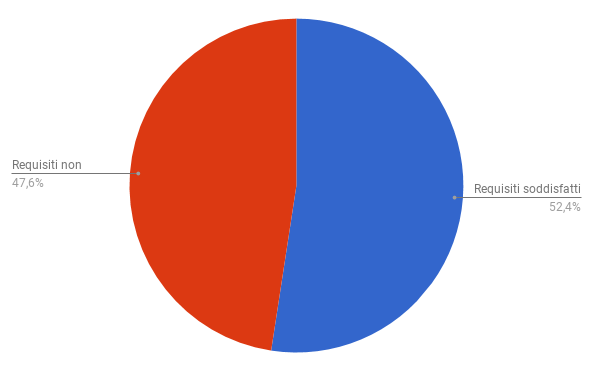
\includegraphics[height=7cm]{img/RequisitiSoddisfatti.png}\\
\caption{Requisiti soddisfatti}
\end{figure}

\begin{figure}[hp]
\centering
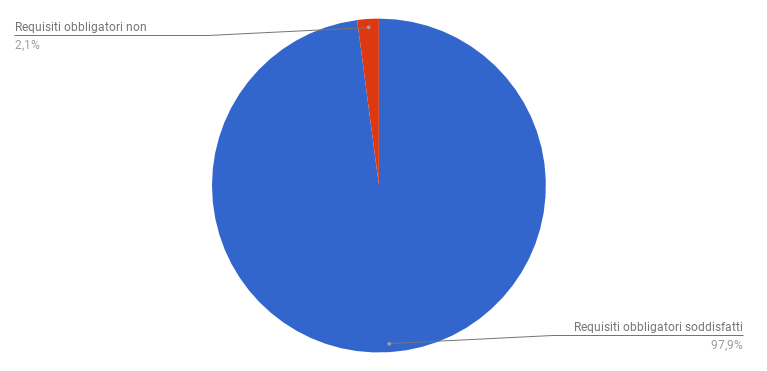
\includegraphics[height=7cm]{img/RequisitiObbligatoriSoddisfatti.png}\\
\caption{Requisiti obbligatori soddisfatti}
\end{figure}
